\chapter{Opis działania aplikacji}

Szczegółowe przedstawienie mechanizmów działania systemu tłumaczy sposób, w jaki dane przemieszczają się między urządzeniami. Ułatwia to zrozumienie logiki aplikacji oraz technicznych aspektów integracji poszczególnych modułów.

\section{Środowisko i struktura projektu}
Podczas prac deweloperskich wykorzystano środowiska IntelliJ IDEA oraz Android Studio. Struktura projektu jest podzielona na niezależne moduły: projekt serwerowy, projekt mobilny oraz pliki frontendu webowego. Baza danych MySQL pracuje jako osobna usługa, co symuluje rzeczywiste warunki pracy systemów sieciowych.

\section{Przepływ danych oraz integracja}
Dane przepływają w systemie w sposób liniowy. Mikrokontroler ESP32 po odczytaniu temperatury formuje paczkę JSON i wysyła ją na endpoint serwera. Serwer Spring Boot przetwarza tę paczkę, dodaje do niej datę i godzinę systemową, po czym wysyła polecenie zapisu do bazy danych. Aplikacje mobilna i webowa w stałych odstępach czasu (co 10 sekund) odpytują serwer o najnowsze dane. Jeśli w bazie pojawiły się nowe rekordy, interfejsy użytkownika są natychmiastowo aktualizowane.

\section{Interfejs użytkownika}

Interfejs mobilny skupia się na czytelności – na pierwszym planie znajduje się karta \\ z ostatnią temperaturą, a poniżej chronologiczna lista wszystkich wpisów. Interfejs webowy prezentuje dane w formie przejrzystej tabeli, która umożliwia wygodną analizę historii pomiarów na ekranie komputera.

Jak pokazano na rysunku \ref{fig:web}, poniżej przedstawiono interfejs webowy do przeglądu danych.
\begin{figure}[H]
    \centering
    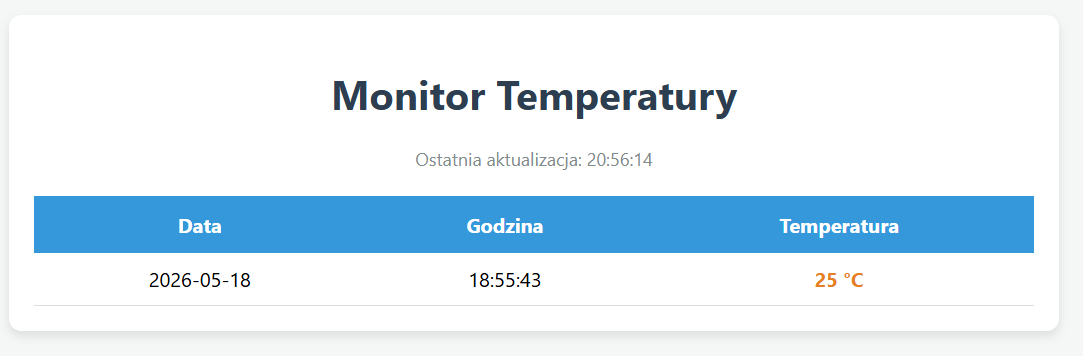
\includegraphics[width=0.7\textwidth]{rysunki/web.png} 
    \caption{Interfejs webowy}
    \label{fig:web} % Klucz dla grafiki PNG
    \sourcefig{opracowanie własne}
\end{figure}
\pagebreak
Jak pokazano na rysunku \ref{fig:app}, poniżej przedstawiono interfejs mobilny aplikacji.
\begin{figure}[H]
    \centering
    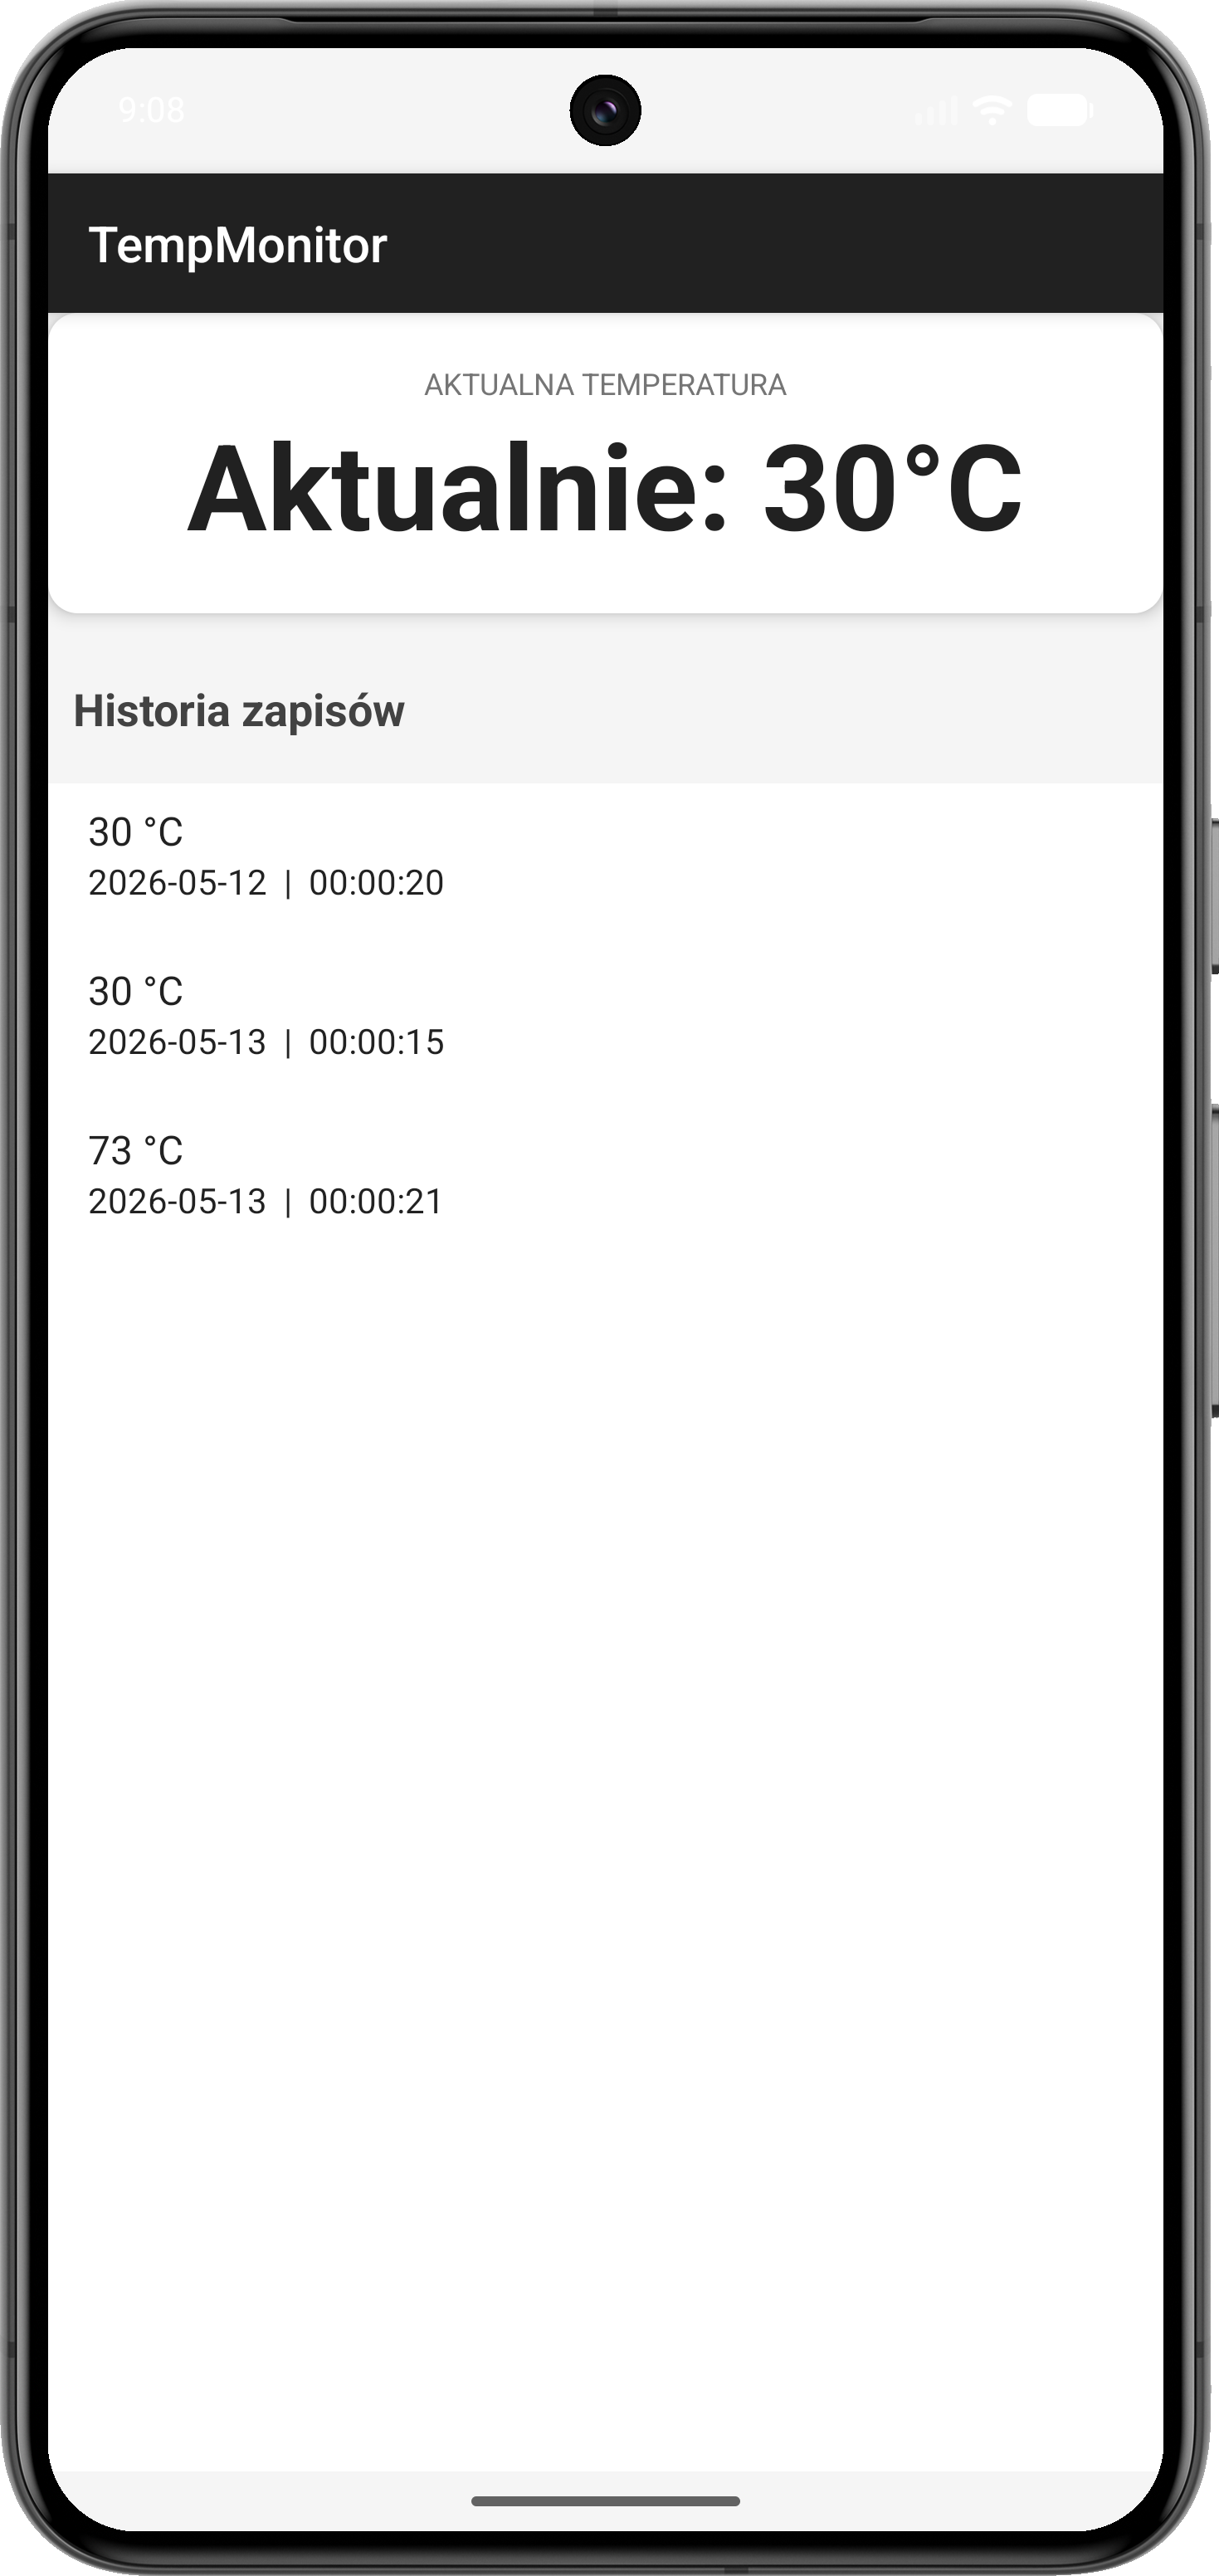
\includegraphics[width=0.6\textwidth]{rysunki/app.png} 
    \caption{Interfejs mobilny}
    \label{fig:app} % Klucz dla grafiki PNG
    \sourcefig{opracowanie własne (Android Studio)}
\end{figure}

\section{Fragmenty kodu źródłowego}